\subsection{RESULTADOS DE LAS DIFERENTES VARIANTES DE LA CADENA}

\subsubsection{Ejemplo de cálculo}
Se calcula el promedio de cada métrica para las diferentes configuraciones propuestas, y se calcula la mejora porcentual. Por ejemplo, para el SNR, el valor promedio calculado en el dataset original es de 19.08 dB. Al analizar el SNR para todas las variantes, se encuentra que el valor mas bajo de SNR es de 19.89 dB, mientras que el valor mas alto es de 33.78 dB. Las resultados ordenados según el porcentaje de mejora se puede ver en Tabla \ref{tab:snr-improvement}.

\begin{table}[h]
\centering
\small
\caption{Mejora SNR por métrica de calidad y algoritmo de denoising.}
\label{tab:snr-improvement}
\begin{tabular}{@{} l l r @{}}
\toprule
\shortstack{\textbf{Filtro de calidad}\\\textbf{y umbral}} &
\shortstack{\textbf{Algoritmo}\\\textbf{de denoising}} &
\shortstack{\textbf{Mejora}\\\textbf{SNR (\%)}} \\
\midrule
NISQA = 3    & Sin denoising    & 4.07 \\
NISQA = 3.5  & Sin denoising    & 4.93 \\
DNSMOS = 2.7 & Sin denoising    & 6.93 \\
DNSMOS = 3.4 & Sin denoising    & 7.56 \\
DNSMOS = 3.0 & Sin denoising    & 9.92 \\
DNSMOS = 3.2 & Sin denoising    & 10.00 \\
NISQA = 3.8  & Deepfilternet    & 10.13 \\
NISQA = 4.2  & Sin denoising    & 11.67 \\
DNSMOS = 3.4 & Deepfilternet    & 12.52 \\
NISQA = 3.5  & Deepfilternet    & 14.78 \\
NISQA = 3.8  & Sin denoising    & 15.58 \\
DNSMOS = 3.2 & Deepfilternet    & 15.65 \\
NISQA = 3.0  & Deepfilternet    & 15.72 \\
NISQA = 4.2  & Deepfilternet    & 17.55 \\
DNSMOS = 3.0 & Deepfilternet    & 17.86 \\
DNSMOS = 2.7 & Deepfilternet    & 18.84 \\
DNSMOS = 3.4 & Demucs           & 39.66 \\
NISQA = 4.2  & Demucs           & 40.34 \\
NISQA = 3.8  & Demucs           & 40.54 \\
NISQA = 3.5  & Demucs           & 41.24 \\
DNSMOS = 3.2 & Demucs           & 41.78 \\
NISQA = 3.0  & Demucs           & 42.16 \\
DNSMOS = 3.0 & Demucs           & 43.25 \\
DNSMOS = 2.7 & Demucs           & 43.52 \\
\bottomrule
\end{tabular}
\end{table}

Este análisis es el que se pondera para cada variable en las 4 categorías de métricas propuestas.

\subsubsection{Métricas separadas}
En una instancia exploratoria previa a la definición de la métrica conjunta, se exploran los resultados del dataset de prueba ante las diferentes métricas propuestas.

Primero es compara la relación entre calidad de audio y cantidad de horas del dataset. La Figura \ref{fig:horas_vs_pesq} muestra, en el eje horizontal, el porcentaje de reducción del dataset producido por el filtrado (más a la derecha significa pérdida de más horas) y, en el eje vertical, el incremento relativo de la puntuación PESQ expresado en porcentaje. Sobre la misma gráfica se comparan las tres variantes de la etapa de realce consideradas: DeepFilterNet, Demucs y la condición sin denoise. El comportamiento observado evidencia un trade-off claro entre cantidad y calidad: umbrales de filtrado más estrictos producen mejoras mayores en PESQ pero sacrifican un mayor número de horas de grabación. En concreto, las variantes con denoising aportan ganancias moderadas en PESQ (típicamente inferiores al 8\% según el umbral), mientras que la variante sin realce logra aumentos mayores en PESQ (superiores al 10\%) a costa de una reducción de dataset mucho más agresiva. Entre los métodos de realce usados, Demucs tiende a ofrecer las mayores mejoras de PESQ a lo largo de los umbrales evaluados, y DeepFilterNet presenta ganancias más pequeñas para filtros equivalentes; esta diferencia implica que la elección del algoritmo de realce y del umbral de NISQA debe hacerse en función del balance deseado entre calidad perceptual y preservación de horas útiles.

\begin{figure}[h]
  \centering
  \centerline{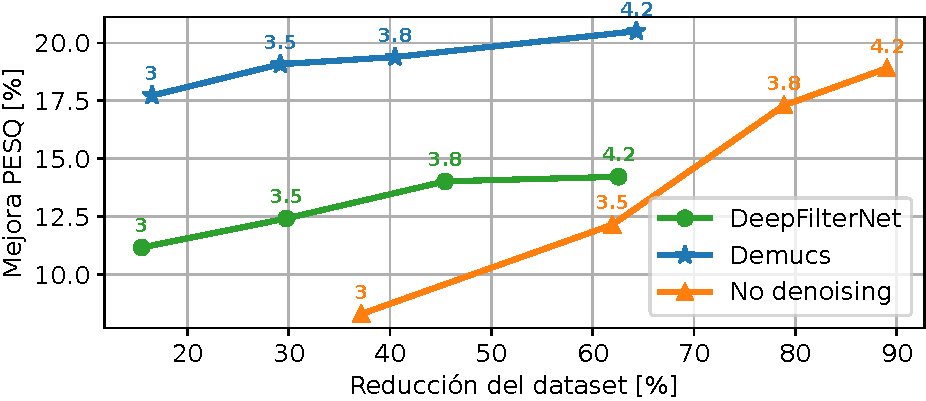
\includegraphics[width=12cm]{Figuras/Pipeline/PESQ vs horas (nisqa).pdf}}
  \caption{Comparación entre PESQ y cantidad de horas de diferentes variantes con NISQA.}
    \label{fig:horas_vs_pesq}
\end{figure}

En la Figura \ref{fig:T30_vs_horas} se relaciona la reducción porcentual de horas con la mejora relativa en \(T_{30}\) (tiempo de reverberación estimado) cuando se emplea DNSMOS como métrica de filtrado. En la gráfica, un aumento en la mejora de \(T_{30}\) implica una reducción de la energía tardía y, por ende, una menor reverberación aparente en los segmentos retenidos. Los resultados muestran que el filtrado aporta ganancias en condiciones sin denoise de forma especialmente notable, cuando no se aplica realce previo el filtrado selecciona segmentos con menor reverberación y la mejora en \(T_{30}\) es sustancial. En cambio, en las condiciones ya denoised las ganancias en \(T_{30}\) son más moderadas (por debajo aproximadamente del 5\% en los umbrales considerados). Además, no se detecta una diferencia significativa en \(T_{30}\) entre DeepFilterNet y Demucs. En conjunto, la figura subraya que el filtrado basado en DNSMOS puede reducir la reverberación del subconjunto resultante, pero el beneficio marginal depende fuertemente de si previamente se aplicó un algoritmo de realce y de la agresividad del umbral.

\begin{figure}[h]
  \centering
  \centerline{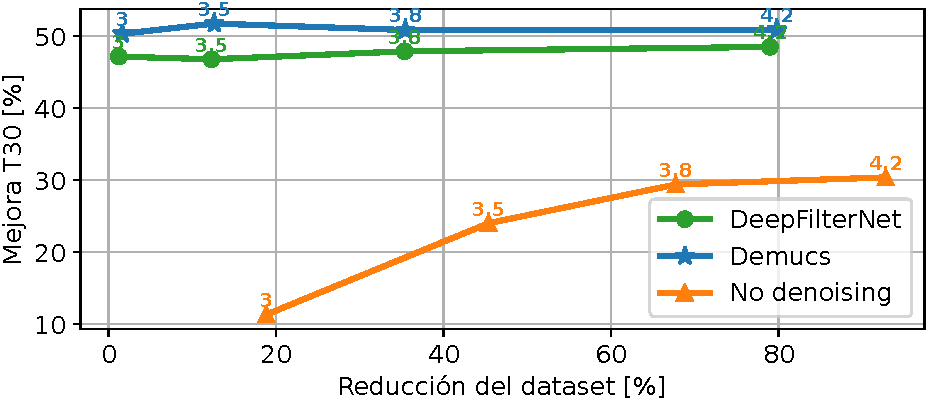
\includegraphics[width=12cm]{Figuras/Pipeline/T30 vs horas (dnsmos).pdf}}
  \caption{Comparación entre T30 y cantidad de horas de diferentes variantes con DNS MOS.}
    \label{fig:T30_vs_horas}
\end{figure}

Además, de comparar la cantidad de horas, también se pueden relacionar otras variables, como puede ser la desviación de frecuencia fundamental \(F0\text{-}STD\) y la mejoría de calidad cuantificada por PESQ Figura \ref{fig:F0_vs_PESQ}. En este análisis se ilustra la relación entre la mejora relativa de PESQ (eje horizontal) y la diferencia porcentual en la desviación estándar de \(F0\) (\(F0\text{-}STD\), eje vertical) para las variantes evaluadas con DNSMOS. Esta representación revela un efecto colateral relevante: a medida que aumenta la mejora perceptual (PESQ) por filtrado más estricto, suele observarse una reducción de la variabilidad prosódica medida por \(F0\text{-}STD\). La explicación práctica es que el filtrado agresivo tiende a eliminar segmentos y hablantes de peor calidad, lo cual reduce la heterogeneidad prosódica del subconjunto retenido. No obstante, los métodos de realce que mejor preservan el timbre de voz muestran cambios menores en \(F0\text{-}STD\) ante el mismo grado de filtrado, lo que indica que ciertos denoisers permiten mejorar la calidad percibida sin sacrificar tanto la variabilidad prosódica. En la práctica, la figura pone de manifiesto el compromiso entre mejorar la calidad objetiva del audio y mantener la diversidad de patrones de entonación: selección excesiva orientada únicamente a PESQ puede empobrecer la variabilidad del corpus, con posible impacto en tareas de síntesis que requieran conservar rasgos prosódicos y de identidad.

\begin{figure}[h]
  \centering
  \centerline{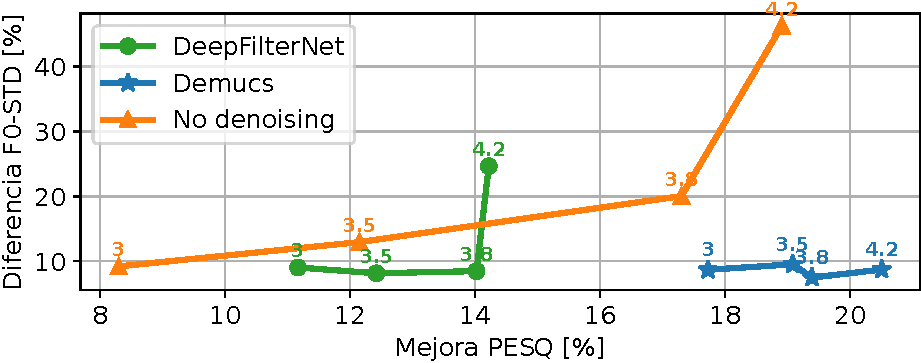
\includegraphics[width=12cm]{Figuras/Pipeline/F0-STD vs PESQ (nisqa).pdf}}
  \caption{Comparación entre F0-std y PESQ para diferentes variantes con DNS MOS.}
    \label{fig:F0_vs_PESQ}
\end{figure}

Este análisis pone en evidencia las relaciones de compromiso entre las métricas seleccionadas y como la mejor variante no será la que alcance un mejor resultado en particular, sino la que logre un mejor balance de todos los criterios en conjunto.

\subsubsection{Métricas compuestas}
Una vez validado el comportamiento de cada métricas de forma individual, se analiza las métricas compuestas definidas en la Sección \ref{sec:metricas_description}. Primero, la calidad de la señal, presenta el comportamiento similar a la tendencia explicada al analizar PESQ. Esto es evidente, ya que tanto PESQ, SI-SDR y SNR sigen la misma tendencia, como se presenta en las gráficas completas en el Anexo A.

En la Figura \ref{fig:RD_vs_CS}, se compara la métrica compuesta de reducción de datos (RD), respeto a la calidad de la señal (CS). Como la métrica se diseñó para minimizar el objetivo total, se puede ver que el mínimo coincide con la variante que filtra menor cantidad de datos y utiliza Demucs como algoritmo de denoising, resultado que coincide con el análisis de las métricas de forma aislada.

\begin{figure}[h]
  \centering
  \centerline{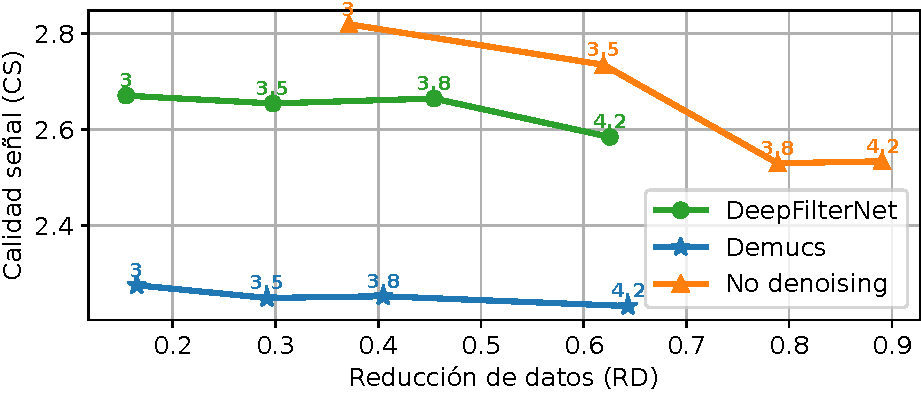
\includegraphics[width=12cm]{Figuras/Pipeline/RD vs CS (nisqa).pdf}}
  \caption{Comparación entre reducción de datos y calidad de señal para diferentes variantes con Nisqa.}
    \label{fig:RD_vs_CS}
\end{figure}

Se analizaron y compararon todas las combinaciones de las diferentes métricas. Los resultados completos de este análisis se presentan en el Anexo B. Los resultados mas destacados son la comparación entre...
(ver de los gráficos los resultados mas importantes pasarlos acá arriba)

\subsubsection{Optimización de la cadena}
Al sumar todas las métricas compuestas, se obtiene la métrica conjunta o total, con la cual se puede ordenar las variantes de la cadena y así definir cual es la configuración optima para procesar un conjunto de datos del habla.

En la Tabla \ref{tab:metricas_ranking}, se presenta el valor de cada métricas compuesta y el valor de la métrica conjunta, para todas las variantes, ordenadas de menor a mayor (siendo el mínimo la mejor variantes y máximo la pero variante).

\begin{table}[ht]
\centering
\small
\caption{Métricas compuestas y total para todas las configuraciones.}
\label{tab:metricas_ranking}
\begin{tabular}{@{} l S l S[table-format=1.2] S[table-format=1.2] S[table-format=1.2] S[table-format=1.2] S[table-format=1.2] @{}}
\toprule
Filtrado & {Umbral} & Denoiser & {RD} & {CS} & {CA} & {DH} & {TOT} \\
\midrule
Dnsmos  & 2.7 & Demucs        & 0.02 & 2.30 & 1.29 & 0.48 & \textbf{4.08} \\
Dnsmos  & 3.0 & Demucs        & 0.13 & 2.27 & 1.27 & 0.51 & 4.17 \\
Nisqa   & 3.0 & Demucs        & 0.17 & 2.28 & 1.27 & 0.60 & 4.31 \\
Nisqa   & 3.5 & Demucs        & 0.29 & 2.25 & 1.28 & 0.58 & 4.41 \\
Nisqa   & 3.8 & Demucs        & 0.40 & 2.25 & 1.30 & 0.55 & 4.51 \\
Dnsmos  & 3.2 & Demucs        & 0.35 & 2.25 & 1.27 & 0.63 & 4.51 \\
Dnsmos  & 2.7 & DeepFilterNet & \textbf{0.01} & 2.66 & 1.37 & 0.62 & 4.65 \\
Nisqa   & 4.2 & Demucs        & 0.64 & \textbf{2.22} & 1.29 & 0.52 & 4.68 \\
Dnsmos  & 3.0 & DeepFilterNet & 0.12 & 2.63 & 1.37 & 0.61 & 4.73 \\
Nisqa   & 3.0 & DeepFilterNet & 0.15 & 2.67 & 1.37 & 0.63 & 4.83 \\
Dnsmos  & 3.2 & DeepFilterNet & 0.35 & 2.62 & 1.35 & 0.60 & 4.93 \\
Dnsmos  & 2.7 & No denoising  & 0.19 & 2.85 & 1.82 & \textbf{0.07} & 4.93 \\
Nisqa   & 3.5 & DeepFilterNet & 0.30 & 2.65 & 1.38 & 0.63 & 4.96 \\
Dnsmos  & 3.0 & No denoising  & 0.45 & 2.72 & 1.66 & 0.12 & 4.96 \\
Dnsmos  & 3.4 & Demucs        & 0.80 & 2.23 & \textbf{1.24} & 0.78 & 5.05 \\
Nisqa   & 3.0 & No denoising  & 0.37 & 2.82 & 1.79 & 0.09 & 5.08 \\
Dnsmos  & 3.2 & No denoising  & 0.68 & 2.65 & 1.58 & 0.20 & 5.10 \\
Nisqa   & 3.8 & DeepFilterNet & 0.45 & 2.66 & 1.37 & 0.64 & 5.13 \\
Nisqa   & 3.8 & No denoising  & 0.79 & 2.53 & 1.69 & 0.20 & 5.21 \\
Nisqa   & 3.5 & No denoising  & 0.62 & 2.74 & 1.74 & 0.13 & 5.22 \\
Dnsmos  & 3.4 & DeepFilterNet & 0.79 & 2.59 & 1.32 & 0.58 & 5.29 \\
Nisqa   & 4.2 & DeepFilterNet & 0.63 & 2.58 & 1.37 & 0.81 & 5.39 \\
Dnsmos  & 3.4 & No denoising  & 0.93 & 2.65 & 1.54 & 0.28 & 5.39 \\
Nisqa   & 4.2 & No denoising  & 0.89 & 2.53 & 1.65 & 0.46 & 5.53 \\
\bottomrule
\end{tabular}
\end{table}

La mejor configuración es la que utiliza XXXX, que obtiene un valor total de 4.5, mientras que la peor variante alcanza un valor total de 5.
Es interesante analizar como la mejor variante, no es la mejor opción en ninguna de las métricas compuestas, sino que ofrece la mejor relación de compromiso entre las 4 condiciones evaluadas.


\subsubsection{Análisis del peso de cada métrica}
Se analiza la varianza de cada métrica en función de las distintas configuraciones para determinar cual métrica tiene mas peso en el ordenamiento propuesto por la metodología de evaluación.

\subsection{COMPARACIÓN ENTRE CONJUNTOS DE DATOS}
Comparar entre conjuntos de datos profesionales vs datos ITW (por parámetros acústicos)

\subsection{COMPARACIÓN POR ESTIMACIÓN DE DENSIDAD}
Comparar entre conjuntos de datos profesionales vs datos ITW (por estimación de densidad)

\subsection{VALIDACIÓN MODELO DE TTS ZERO-SHOT}
Compara calidad de clonación respecto a la calidad o subset del audio original
